

\section{Outline of our approach}
\label{s:outline}
 
In this Section we outline our approach:  
we  revisit  our running example, the Bank Account (\S\ref{s:bank}),  
introduce the three necessity operators (\S \ref{s:approach:necopers}),  give 
the \Nec specs (\S \ref{s:bankSpecEx}),
   outline how we model the open world (\S\ref{s:concepts}), 
give the main ideas of our proof system (\S\ref{s:approach})
and   outline 
how we use it to reason 
about adherence to \Nec specifications  (\S\ref{s:all:outline:proof}).
 

 \subsection{Bank Account -- three modules}
\label{s:bank}
  
Module \ModA consists of an empty 
\prg{Password} class where each instance models a unique password, and an  \prg{Account} class with a password, and a balance, an \prg{init} method to 
initialize the password, and 
a
\prg{transfer} method. 
\sdS{Note that we assume that all  fields are  ``class-private'', 
i.e., methods may read and write fields of any instance of the same class,
and  that passwords are unforgeable and not enumerable (as
in Java, albeit without reflection}.
%
% 
\begin{lstlisting}[mathescape=true, language=Chainmail, frame=lines]
module $\ModA$
  class Account
    field balance:int 
    field pwd: Password
    method transfer(dest:Account, pwd':Password) -> void
      if this.pwd==pwd'
        this.balance-=100
        dest.balance+=100
     method init(pwd':Password) -> void
      if this.pwd==null
        this.pwd=pwd'
  class Password
\end{lstlisting}
%
\noindent 
We can capture the intended semantics of   \prg{transfer}  
through  {a}  \funcSpec with pre- and post- conditions and \prg{MODIFIES} clauses as \emph{e.g.,} in \citeauthor{Leavens-etal07,dafny13}.
The implementation of  \prg{transfer} in module  $\ModA$ meets
this specification.

\begin{lstlisting}[mathescape=true, frame=lines, language=Chainmail]
$\Sclassic$  $\triangleq$
   method transfer(dest:Account, pwd':Password) -> void  
      ENSURES:
            this.pwd$=$pwd' $\wedge$ this$\neq$dest  $\longrightarrow$  
            this.balance$_{post} =$this.balance$_{pre}$-100 $\wedge$ dest.balance$_{post} =$dest.balance$_{pre}$+100
      ENSURES:
            this.pwd$\neq$pwd' $\vee$ this$=$dest  $\longrightarrow$ 
            this.balance$_{post} =$this.balance$_{pre}$ $\wedge$ dest.balance$_{post} =$dest.balance$_{pre}$ 
      MODIFIES:  this.balance, dest.balance        
\end{lstlisting}
 
 
Now consider the following alternative implementations:
\ModB allows any client to reset an account's password at any time;
\ModC requires the existing password in order to change it.
  
  

\begin{tabular}{lll}
\begin{minipage}[b]{0.42\textwidth}
\begin{lstlisting}[mathescape=true, language=chainmail, frame=lines]
module $\ModB$
  class Account
    field balance:int 
    field pwd: Password 
    method transfer(..) ...
      ... as earlier ...
    method init(...) ...
       ... as earlier ...
    method set(pwd': Password)
      this.pwd=pwd'
      
  class Password
\end{lstlisting}
\end{minipage}
&\ \ \  \ \   &%
\begin{minipage}[b]{0.45\textwidth}
\begin{lstlisting}[mathescape=true, language=chainmail, frame=lines]
module $\ModC$
  class Account
    field balance:int 
    field pwd: Password 
    method transfer(..) 
      ... as earlier ...
    
    
    method set(pwd',pwd'': Password)
      if (this.pwd==pwd') 
        this.pwd=pwd''
  class Password
\end{lstlisting}
\end{minipage} 
\end{tabular}

Although the \prg{transfer} method is the same in
all three alternatives, and each one satisfies \Sclassic,
code  {such as}
\\ 
$\ \strut \hspace{.2in} $ \prg{an\_account.set(42); an\_account.transfer(rogue\_account,42)}
\\ 
is enough to drain  \prg{an\_account} in \ModB without knowing the password.

\sdS{This example also demonstrates the importance of field privacy: $\ModA$ and $\ModC$ would not be any
more robust than $\ModB$ if the underlying programming language did not restrict access to fields. Without 
such a restriction,
any external object would have been able to directly manipulate the fields \prg{balance} and \prg{pwd}}.

\subsection{The three necessity operators}
\label{s:approach:necopers}

{We need  a specification that rules out \ModB while permitting \ModA and
\ModC.  For this, we will be using  one of the  three necessity operators mentioned in  \S \ref{intro:this:work}. These operators are:}
\\
$ \strut \hspace{1.7in} \onlyIf {A_{curr}} {A_{fut}} {A_{nec}} $ \\
$ \strut \hspace{1.7in}   \onlyIfSingle {A_{curr}} {A_{fut}} {A_{nec}} $ \\
$ \strut \hspace{1.7in}   \onlyThrough {A_{curr}} {A_{fut}} {A_{intrm}} $
%\strut \hspace{.4in} \onlyIfSingle {A_{curr}} {A_{fut}} {A_{nec}}. \strut \hspace{.4in} \onlyThrough {A_{curr}} {A_{fut}} {A_{intrm}}
\\
The first operator was already introduced in \S \ref{intro:this:work}: it says that  
a  {transition} from a current state satisfying assertion $A_{curr}$ to a future
state satisfying $A_{fut}$  is possible only if  the   necessary 
condition
$A_{nec}$ holds in the \emph{current} state.
%
{The  second operator says    that 
a  \emph{one-step} {transition} from a current state satisfying assertion $A_{curr}$ to a future
state satisfying $A_{fut}$  
is possible only if % the   necessary condition
$A_{nec}$ holds in the \emph{current} state.   
The   third operator   says that a change from %a current state satisfying 
 $A_{curr}$ to  $A_{fut}$  may happen only if % the necessary condition
 $A_{intrm}$ holds in some \emph{intermediate} state.}
 
  
%  \vspace{.02in}
%  
%Unlike  \emph{Chainmail}'s temporal operators, 
% the necessity operators %  $\onlyIf {\_} {\_} {\_}$  and $\onlyThrough {\_} {\_} {\_}$
% are  not first class, and may not appear in the assertions  {(\eg  ${A_{curr}}$)}. 
% This simplification enabled us to develop our proof logic. 
% Thus, we {have reached} a  sweet spot between expressiveness and 
% provability.

{
Our assertions $A$, also allow for the use of capability operators, such as 
1) having \prg{access} to an object ($\access{\prg{o}}{\prg{o'}}$) which means that $\prg{o}$ has a reference to $\prg{o'}$,
 or 2) \prg{calling} a method with on receiver with certain arguments, 
  ($\calls{\prg{o}}{\prg{o'}}{\prg{m}}{\prg{args}} $), or 3) an object being \prg{external},
  where  $\external{\prg{o}}$ means that \prg{o} belongs to a class that is not defined in the current module,
  and thus its behaviour is unrestricted.}
 These are the capability operators that we have 
adopted from Chainmail.


 \subsection{Bank Account -- the right specification}
\label{s:bankSpecEx}

We now {return to our quest for} a specification that rules out \ModB while permitting \ModA and
\ModC. The catch is that the vulnerability present in \ModB is the result
of  \emph{emergent} behaviour from the interactions of the \prg{set}
and \prg{transfer} methods --- even though \ModC also has a
\prg{set} method, it does not exhibit the unwanted interaction.
This is exactly where a necessary condition can help:
we want to avoid transferring money
(or more generally, reducing an account's balance)
\textit{without} the existing account password.  Phrasing the same condition
the other way around % gives us a positive statement that still
rules out the theft: that money \textit{can only} be
transferred when the account's password is known.


In \Nec  syntax, and {recalling \S \ref{intro:this:work}, and \ref{s:approach:necopers},}
 

%
%% The flaw in version {\sf{II}} arises from 
%% can be used to overwrite the
%% password, and then using the new password \prg{transfer}  can be called.
% If we want the \prg{Account} class to be robust, we must prohibit the password from being freely available.
%
%
%% In this paper, we show how \textit{necessity specifications} can solve
%% this progkem.  
%%  Therefore, we propose a %holistic 
%%  specification which says that
%%  the \prg{balance} of an \prg{Account} reduces only if an object which does not belong to the
%%  module has access to the password:
%
%
 %% Therefore, we propose a %holistic 
 %% specification which says that
 %% the \prg{balance} of an \prg{Account} reduces only if an object which does not belong to the
 %% module has access to the password:
%
\begin{lstlisting}[language = Chainmail, mathescape=true, frame=lines]
   $\text{\SrobustA}$  $\triangleq$   from   a:Account $\wedge$ a.balance==bal    next    a.balance < bal
                onlyIf $\exists$ o,a'. [$\external{\prg{o}}$ $\wedge$ $\calls{\prg{o}}{\prg{a}}{\prg{transfer}}{\prg{a'},\prg{a.pwd}} $]    
                
   $\text{\SrobustB}$  $\triangleq$   from   a:Account $\wedge$ a.balance==bal    to    a.balance < bal
                onlyIf $\exists$ o.[$\external{\prg{o}}$ $\wedge$ $\access{\prg{o}}{\prg{a.pwd}}$]    
           
\end{lstlisting}
%
%
% 
%% In more detail, the specification from above says that if in the current
%% configuration \prg{a} is an \prg{Account},
%% and in some future configuration \prg{a} will have a balance less than the current one, then,in the \emph{current} configuration
%% there must exist some object \prg{o}, which is \emph{external} to our module (does not belong to module
 %% \prg{AccountMdl}), and which has access to \prg{a}'s password.
 %
%% T9hu having access to the password is a necessary condition for the balance to reduce.

 
{\SrobustA does not fit the bill: all three modules   satisfy  it.
 % \SrobustA;  this demonstrates that \SrobustA is not strong enough. 
 But  \SrobustB does fit the bill: \ModA and \ModC satisfy \SrobustB, while \ModB does not.}
 
A critical point of \SrobustB % this \Nec specification 
is that it is
expressed in terms of observable effects (the account's balance is
reduced: \prg{a.balance < bal}) and the shape of the heap 
(external access to the password:
$\external{\prg{o}}\ \wedge\ \access{\prg{o}}{\prg{a.pwd}}$) 
rather than in terms of individual methods such as
\prg{set} and \prg{transfer}.
This gives our specifications the
vital advantage that they can be used to constrain
\jm[typo]{\textit{implementations}} of a bank account with a balance and a
password, irrespective of the API it
offers, the services it exports, or the dependencies on other parts of
the system.

 This example also demonstrates that 
adherence to   \Nec specifications is not monotonic:
adding a method to a module does not necessarily preserve adherence to
a specification, 
and while separate methods may adhere to a  specification, their combination does
not necessarily do so. 
{For example, \ModA satisfies \SrobustB, while \ModB does not.}
This is why we say that \Nec   specifications capture a module's \emph{emergent behaviour}. 
 

%\jm[TODO: in the proof later we need to mention that there is a difference between the overall proof (no mention of the methods), and the intermediate ones (that do mention the methods)]{}
\subsubsection{How  useful is  \SrobustB?}
\label{sec:how}

{One might think that \SrobustB was not useful: normally, there will exist somewhere in the heap
at least one external object  
with access to the password --  if no such object existed, then \sdN{nobody} would be able to use the money of
the account.
And if such an object did exist, \sdN{then the premise of \SrobustB would not hold, and thus}
the guarantee given by \SrobustB might seem vacuous.}

{
This is \emph{not} so: %there may exist  
\sdN{in scopes   from which such external objects with access to the password
are not (transitively) reachable, % . In such scopes,
\SrobustB  guarantees that the balance of the account will not decrease.
}
We illustrate this through the following  code snippet:
 

\begin{lstlisting}[mathescape=true, language=chainmail, frame=lines]
module $\ModParam{1}$
     ...
    method cautious(untrusted:Object)
        a = new Account
        p = new Password
        a.set(null,p)
        ...
        untrusted.make_payment(a)
        ...
\end{lstlisting}
 

{The method \prg{cautious} has as  argument an external object \prg{untrusted}, of unknown provenance.
{It} creates a new \prg{Account} and initializes its password. 
In the scope of  this method,  external objects with access to the password are reachable:
thus,  during execution of  line 7, or   line {9} the balance may decrease.
}

{Assume that class \prg{Account} is from a module which satisfies \SrobustB. 
Assume also that the code in line 7 does not leak the password to \prg{untrusted}. Then no external object
reachable from the scope of execution of \prg{make\_payment} at line 8 has access to the password.
Therefore, 
even though we are calling   an untrusted object, \SrobustB guarantees that \prg{untrusted}
 will not be able to take any money out of  \prg{a}.
 }
 
\jm[]{
A  proof sketch of the  safety provided by \SrobustB appears in Appendix \ref{app:safety}.
}
\sdN{Note that in this example, we have (at least) three modules: the internal module 
which defines class \prg{Account} adhering to  \SrobustB, the  
external module $\ModParam{1}$, and the external module which contains the class definition for \prg{untrusted}.
Our methodology allows the external module, $\ModParam{1}$ to reason about its own code, and thus 
pass \prg{a} to code from the second external module, without fear of losing money.}
\sdN{In further work we want to make such arguments more generally applicable, and 
extend Hoare logics to encompass such proof steps.}
%\susan[I think this paragraph doesn't add, if anything it has a hostage to fortune. I would just remove it.
% The purpose of the current paper is being able to express specifications like \SrobustB, and
%and being able to prove adherence. In further work we want to develop logics to leverage such specifications, putting
%informal arguments as the  one of this section onto formal foundations.
 
 

 
\subsection{Internal and external modules, objects, and calls}
\label{s:concepts}

Our work concentrates on guarantees made in an \emph{open} setting; that is, a given module
$M$ must be programmed so that 
execution of $M$ together with \emph{any} \externalM 
module $M'$ will uphold these guarantees. In the tradition of
visible states semantics, we are  only interested in upholding the guarantees while 
$M'$, the  \emph{\externalM} module, is executing. A module can
temporarily break its own invariants,
so long as the broken invariants are never visible externally.
   
We therefore distinguish between  \emph{\internalO}
objects --- instances of classes defined in $M$ ---
and \emph{\externalO} objects defined in any other module.
We also distinguish between
  \emph{\internalC} calls  (from either an internal or an external object)  made % from \externalO objects
 to \internalO objects and \emph{\externalC} calls made % from \externalC objects
 to \externalC objects. 
{Looking at the code snippet from \S \ref{sec:how}, the call to \prg{set} on line 6 is an 
 internal call, while the call to \prg{make\_payment} is an external call -- from the external 
 object  \prg{this}  to the external object \prg{untrusted}.}
 
 % We are less
% interested in calls made from \internalO objects to \internalO objects, because we only need 
% establish the guarantees when the \externalM module is executing. And we 
%
%
Because we only require guarantees while 
the  \externalM module  is executing,
we develop an \emph{external states} semantics, where
 any internal calls are executed in one, large, step.
With external steps semantics,  the executing object (\prg{this}) is always   external. 
  In line  with other work in the literature \cite{Permenev, Grossman, Albert}, we currently forbid 
  calls from internal to  external objects
  -- further details on call-backs in \S\ref{s:related}. 

{For the purposes of the current work we are only interested in one internal, and one external module.
But the interested reader might ask: what if there is more than one external module?
The answer is that from the internal module's viewpoint, all external modules are considered as one;
for this we provide a module linking operator with  the expected semantics -- more details in Def. \ref{def:pair-reduce} and \S \ref{app:loo}. 
But from the external module's viewpoint, there may be more than one external module: for example, in \S \ref{sec:how}, 
module $\ModParam{1}$ is external to the module   implementing class \prg{Account}, and the module 
implementing the class of \prg{untrusted} is external to
$\ModParam{1}$.
}

%\section{Encapsulation}
%\label{s:outline:encapsulation}
%\jm[]{\Nec depends upon the encapsulation of data, or more
%specifically the encapsulation of assertions about encapsulated 
%data. We say that an assertion $A$ is encapsulated by module $M$ if $A$ may only
%be invalidated through computation internal to $M$. 
%For example, the assertion \prg{a:Account $\wedge$ a.pwd = p} is
%encapsulated by \ModA (along with \ModB and \ModC) as 
%it requires a write to \prg{a.pwd} and thus may only be invalidated 
%by a call to a method belonging to \ModA.
%}
%
%\jm[]{
%Encapsulation is a topic that is well covered in the literature,
%and as such we build upon that existing work to derive these
%encapsulation guarantees. For the purposes of the examples in this
%paper we define a simple system inspired by confinement types~\cite{confined}, 
%but \Nec could just as easily be 
%}

\newcommand{\vertsp} {\vspace{.05in}} 
 
\subsection{Reasoning about \Nec}
\label{s:approach}

{We will now outline the key ingredients of  our logic with which we prove
that modules obey \Nec specifications. 
We will use the auxiliary concept that  
an assertion $A$ is \emph{encapsulated} by
a module $M$, if  $A$  can only be invalidated through 
a call to a method from $M$ -- more   in \S \ref{s:encaps-proof}.}

 
% is built on top of   
% two existing and widely studied topics:
% \funcSpecs and encapsulation. That is, we assume the existence of
% some proof logic for proving traditional pre- and post-conditions for functions, 
% along with a property we refer to as \emph{assertion encapsulation}.
% We say that an assertion is \emph{encapsulated} if \sophiaPonder[no need for "and only if"]{} invalidation 
% of that assertion by program execution requires a method call to the 
% \emph{internal} module. We discuss assertion encapsulation in more detail in \S \ref{s:encaps-proof}.
% 
%  (1) if an assertion $A$ is encapsulated by a module $M$, then a call to $M$ is a \emph{necessary} pre-condition to invalidating $A$,
% and (2) that the specification $\onlyIf{A_1} {A_2} {A_3}$ is 
%logically equivalent
%% with 
%{to}

The \Nec logic is based on the {insight} that the specification\\
\strut $\hspace{1in}$  $\onlyIf{A_1} {A_2} {A_3}$
\\
 is  logically equivalent {to} \\
 \strut $\hspace{1in}$  $\forall \prg{stmts}. \{ A_1 \wedge \neg A_3\} \prg{stmts} \{ \neg A_2 \}$\\
 -- that is,
 with an \emph{infinite} conjunction  of Hoare triples, \sdS{where the three assertions are fixed, but the code,
 \prg{stmts}, is universally quantified.
This leaves the challenge that \sdr[changed "no Hoare logics support"]{usually, Hoare logics do
 not support} such infinite conjunctions over code.}
 Three \sdr[dropped breakthroughs]{ideas} helped us address   that challenge: 

 \begin{description}
 \item
 [From Hoare triples to per-call specs] 
  The Hoare triple 
$ \{ A_1 \wedge \neg A_3 \} \ \prg{x.m(ys)}\  \{ \neg A_2 \}$ is logically equivalent 
 {to} the specification
$ \onlyIfSingle {(A_1 \wedge  \calls{\_}{\prg{x}}{\prg{m}}{\prg{ys}} )} {A_2} {A_3}$.  
% Thus, we   leverage Hoare triples to \sophiaPonder[it said "reason about" -- I think this was wrong]
% obtain \Nec specs {about specific calls. }   
 
 \item 
 [From per-call specs to per-step specs] % Second, 
 If an assertion $A_2$  is \emph{encapsulated} by a module -- and thus the only way from a 
 state that satisfies $A_2$ to a state that does not, is through a call to a method in that module -- then
{the
\emph{finite conjunction}
that all methods of that module {$ \onlyIfSingle {(\, A_1 \wedge A_2 \wedge {\calls{\_}{\prg{x}}{\prg{m}}{\prg{ys}}}\, )} {\neg  A_2} {A_3}$}
  is logically equivalent 
 {to}
{$ \onlyIfSingle {A_1 \wedge A_2} {\neg A_2} {A_3}$. }}
 
  \item [Proof logic  for emergent behaviour] %an inference system 
  combines several specifications to reason about the
  emergent behaviour, \emph{e.g.,} 
   $ \onlyThrough  {A_1} {A_2} {A_3}$  and $ \onlyIf  {A_1} {A_3} {A_4}$ implies 
   $ \onlyIf  {A_1} {A_2} {A_4}$.
 \end{description}

%\jm[]{Julian Proposal >>>>>>>>>>>>>>>>>>>>>}

%We now outline \sd{our  \Nec logic}.
% and mentioned in \S \ref{intro:this:work} interact with each other.
%\jm[trimmed sentence]{} %to allow us to reason about 
%necessary conditions and emergent behaviour. 
%\Nec logic in this 
%paper is presented bottom up, starting with specifications of individual methods
%in isolation, building up to proofs of emergent behaviour.
%This section outlines the structure of 
%\Nec logic, and follows the 
%We \sd{elaborate further} on the \jm[]{four} breakthroughs  \sd{described} \jm[]{in} %identified in 
%\S\ref{intro:this:work}
%along with two additions: (a) \funcSpecs, and (b) assertion encapsulation. 


  Thus, our system consists of four parts (five including \funcSpecs):
(\textbf{Part 1}) assertion encapsulation, (\textbf{Part 2}) {per-method} specifications, 
(\textbf{Part 3}) per-step specifications, and (\textbf{Part 4}) specifications of emergent behaviour.
The structure of the system, and the dependency of each part on preceding parts is given in Fig. \ref{fig:dependency}.
 \FuncSpecs are used to prove \jm[]{per-method} specifications, which coupled with 
assertion encapsulation is used to prove per-step specifications, which is used to 
prove specifications of emergent behaviour.
\begin{figure}[t]
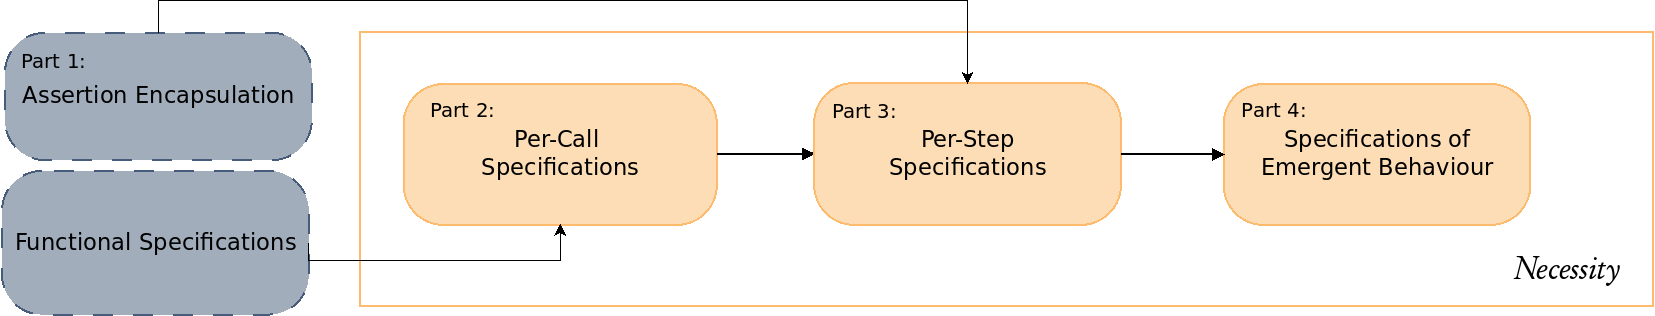
\includegraphics[width=\textwidth]{diagrams/dependency.png}
   \caption{
   Parts of \Nec Logic {and their Dependencies}. 
   Note that gray parts with a dashed border indicate
   parts that are not part of \Nec, and on which \Nec 
   is parametric.}

   \label{fig:dependency}
 \end{figure}

% {\Nec consists of specifications of necessary conditions and a logic for proving those specifications: parts 2, 3, and 4.
%The remaining parts are assertion encapsulation (part 1) and \funcSpecs.
%}
%\jm[]{As previously stated, an} assertion $A$  is
%\emph{encapsulated} by  module $M$, if  $A$ can be invalidated only through
%calls to methods defined in $M$.
%  In other words, a  call to  $M$  is a \emph{necessary} condition for
%invalidation of $A$.
Our \Nec logic  is parametric with respect to  {the way we ascertain whether an assertion
is encapsulated and the way we obtain \funcSpecs.}
As a result we can leverage  results from many different approaches.
Further, our proofs of \Nec do not inspect method
bodies: we rely on simple annotations to infer encapsulation, and
{on} pre and post-conditions  to infer per-method conditions. 

% Because we rely on some external mechanism to obtain \funcSpecs, we never need to inspect method bodies
% when proving \Nec specifications.


%\jm[]{For the purposes of our examples,} \funcSpecs are assumed, and not 
%included as part of the proof system, as they have been well covered in the literature.
%{\jm[]{This is a key strength of our approach:
%\Nec (parts 2, 3, and 4) and our results are } agnostic as to how \jm[]{both assertion encapsulation and \funcSpecs} are proven.
%As a result we can leverage the results of many different approaches.
%Further, our proofs of \Nec do not inspect method
%bodies: we rely on simple annotations to infer encapsulation, and
%\sd{on} pre and post-conditions  to infer per-method conditions. }
 


 
%\jm[]{
%Note that our proofs of necessity do not inspect method
%bodies: we rely on simple annotations to infer encapsulation, and on
%classical pre and postconditions to infer per-method conditions. 
%{Our system is agnostic as to how the pre- and post-conditions are proven,
%and thus we can leverage the results of many different approaches.}
%}
%
%\jm[]{
%\begin{description}
%\item[Part 1: Assertion Encapsulation.] 
%An assertion $A$  is
%\emph{encapsulated} by  module $M$, if  $A$ can be invalidated only through
% % $M$-\internalC calls. 
%calls to methods defined in $M$.
%  In other words, a  call to  $M$  is a \emph{necessary} condition for
%invalidation of $A$.
%Our \Nec logic  is parametric with respect to the 
%particular encapsulation
%mechanism: here we rely on rudimentary annotations inspired by confinement types
%\cite{confined}. More in \S\ref{s:encaps-proof}.
%\item[Part 2: Per-method conditions]   % \emph{per-method-condition}, \ie., a 
%are derived using classical pre- and postconditions on methods.
%As we mention in \S \ref{intro:this:work}, the Hoare triple 
%$\{ A_1 \wedge \neg A_3 \} \ \prg{x.m(ys)}\  \{ \neg A_2 \}$
%is logically equivalent to stating that $A_3$ is a necessary precondition
%for the call \prg{x.m(ys)} with precondition $A_1$ to result in a postcondition $A_2$.
%More in \S\ref{s:classical-proof}.
%%are  necessary conditions for   given  effect and
%%  given single, specified, method call. 
%%To infer these, we  leverage   sufficient conditions 
%%from classical specifications: % Namely, if 
%%If the negation of a method's
%% classical postcondition implies  a given effect, %the effect we are interested in,
%%  then the negation of the 
%% classical precondition  is a necessary precondition for the effect and the method call. 
%%More in \S\ref{s:classical-proof}. 
% \item[Part 3: Single-step conditions] 
%If every method $m$ within a module $M$ has the same necessary condition, 
%$\onlyIfSingle{A \wedge \calls{\_}{x}{m}{ys}}{\neg A}{A_{necc}}$ (from Part 2), and 
%$A$ is encapsulated by $M$ (from Part 1), then it follows that $A_{necc}$ is a necessary precondition
%to invalidate $A$ for \emph{any} possible execution step.
%% are
%% necessary conditions for a given  effect and
%%a single, \emph{unspecified} step. This step could be an internal call, or any kind of external step.
%%    For effects encapsulated by $M$, we can infer such single-step
%% conditions by combining the per-method conditions for that effect from 
%%all   methods in $M$. 
%More in \S\ref{s:module-proof}.
%\item[Part 4: Emergent behaviour] \
%We infer the \emph{emergent} behaviour of a module out of the conditions of \sd{several}
%single steps (from Part 3) using a proof system defined in \S\ref{s:emergent-proof}.
%\end{description}
%}
%
%\jm[]{These parts are dependent on each other, along with an 
%assumed logic for proving classical pre- and postconditions.
%These dependencies are shown in Fig. \ref{fig:dependency}.}
 
 \subsection{Outline of the proof that  \ModC obeys \SrobustB}
 \label{s:all:outline:proof}
 
For illustration, we  outline  a proof that  \ModC adheres to \SrobustB. 
note that for illustration purposes, in this paper we show how assertion encapsulation can be proven
based on simple annotations inspired by confinement types
\cite{confined}; we could just as easily rely  on other language mechanisms,  \emph{e.g.,} ownership types,
{or even develop custom  logics.}
 
\begin{description}
\item[Part 1: Assertion Encapsulation.]  \
%
\vertsp\\
%
{\fbox{\parbox{\linewidth}{
We begin by proving that \ModC encapsulates: %3 properties:
\begin{description}
\item[(A)] The balance
\item[(B)] The password
\item[(C)] External accessibility to an account's password -- 
that is, the property that no external object has access to the password may only 
be invalidated by calls to \ModC.
\end{description}
}}}
% 
\vertsp
% 
\item[Part 2: Per-Method Specifications]   \
%
\vertsp\\
{\fbox{\parbox{\linewidth}{
{We prove} that the call of any  method {from} \ModC (\prg{set} and \prg{transfer}) 
satisfies: % is proven to have the following necessary conditions:
\begin{description}
\item[(D)] If the balance {decreases}, then 
 \prg{transfer} was called with the correct password
\item[(E)] If the password changes, then the method called was
 \prg{set} with the correct password
\item[(F)] It will not provide external accessibility to the password.
\end{description}
}}}
%
\vertsp
%
%
%
\item[Part 3: Per-step Specifications]  \
%
\vertsp \\ 
%
{\fbox{\parbox{\linewidth}{
We then raise our results of Parts 1 and 2 to reason about arbitrary \emph{single-step} executions:
\begin{description}
\item[(F)]
By \textbf{(A)} and \textbf{(D)} only \prg{transfer} and external access to the password may decrease the balance.
\item[(G)]
By \textbf{(B)} and \textbf{(E)} only \prg{set} and external access to the password may change the password.
\item[(H)]
By \textbf{(C)} and \textbf{(F)} no step may grant external accessibility to an account's password.
\end{description}
}}}
%
%\vertsp
%%
%{\fbox{\parbox{\linewidth}{
%Our proof that \textbf{(C2)} does not hold also considers single-step conditions, and takes the following form:
%\begin{description}
%\item[(G)]
%The internal-only access to an account's password is ``encapsulated'', and required internal computation to invalidate.
%\item[(H)]
%No internal method call can be used to coerce access to an account's password.
%\end{description}
%}}}
%  
\vertsp
%
\item[Part 4: Specifications of Emergent Behaviour] \
%
\vertsp \\
%
{\fbox{\parbox{\linewidth}{
We then raise our necessary conditions of Part 3 to reason about \emph{arbitrary} executions:
\begin{description}
\item [(I)]
A decrease in balance over any number of steps implies that some single intermediate step 
reduced the account's balance.
\item [(J)] 
By \textbf{(F)} we know that step must be a call to \prg{transfer} with the correct password.
\item [(K)]
When \prg{transfer} was called, either
\begin{description}
\item[(K1)]
The password used was the current password, and thus by \textbf{(H)} we know that 
the current password must be externally known, satisfying \SrobustB, or
\item[(K2)] 
The password had been changed, and thus by \textbf{(G)} some intermediate step must have been
a call to \prg{set} with the current password. Thus, by \textbf{(H)} we know that
the current password must be externally known, satisfying \SrobustB.
\end{description}
\end{description}
}}}
%
\end{description}


%\noindent\jm[]{\noindent Original >>>>>>>>>>>>>>>>>>>>>}
%
%
%
%We now give a sketch of the novel concepts we developed in  \Nec logic.
%For illustration, we  outline  a proof that  \ModC adheres to \SrobustB.
%
%\begin{description}
%\item[Part 1: Emergent behaviour] \ {is behaviour that arises out 
%of any number of steps and interactions with a module interface.}
%We infer the \emph{emergent} behaviour out of the conditions of  \sd{several}
%single steps.
%This part is crucial;   \sd{for instance,} while \ModB satisfies  
%\SrobustB for one single step, it does not satisfy it for any number of steps. More in \S\ref{s:emergent-proof}.
%
%\vertsp
%%\jm{e.g. In the case of (S3) and \ModB, emergent behaviour refers to the interaction 
%%the \prg{set} method (for setting the password), the \prg{transfer} method, and the account's balance.}
%
%{\fbox{\parbox{\linewidth}{
%Our proof of \sd{\ModC's adherence to \SrobustB} follows the following steps:
%\begin{description}
%\item [(A)]
%A reduction in an account balance over any number of steps implies that some single intermediate step 
%reduced the account's balance.
%\item [(B)] 
%External knowledge of an account's password is a necessary prerequisite to any single step reducing the balance.
%\item [(C)]
%An account's password may only be externally known in the future if either
%\begin{description}
%\item[(C1)]
%the password is currently known externally  thus satisfying \SrobustB, or
%\item[(C2)] it is possible to coerce the internal module interface to expose the password
%\end{description}
%\end{description}
%The proof of (\textbf{B}) is constructed using \textbf{Part 2} and the proof that (\textbf{C2}) does not hold requires us to use the reasoning in \textbf{Part 2} and \textbf{Part 4}.
%}}}
%
%\vertsp 
%
% \item[Part 2: Single-step conditions] are
% necessary conditions for a given  effect and
%a single, \emph{unspecified} step. This step could be an internal call, or any kind of external step.
%  % 
%    For effects encapsulated by $M$, we can infer such single-step
% conditions by combining the per-method conditions for that effect from 
%all   methods in $M$. 
%% We also have  expected sub-structural rules,\eg  like the rule of consequence.
%% Drop above, as we dor 
%More in \S\ref{s:module-proof}.
%
%{\fbox{\parbox{\linewidth}{
%Our proof of \textbf{(B)} considers single-step conditions, and takes the following form:
%\begin{description}
%\item[(D)]
%An account's balance is an ``encapsulated'' property, that requires module internal computation to change.
%\item[(E)]
%The only module internal method call that reduces an account's balance is a call to \prg{transfer} with the account's 
%password.
%\item[(F)]
%An external call to \prg{transfer} with an account's password implies that the password is externally known
%\end{description}
%}}}
%
%\vertsp
%
%{\fbox{\parbox{\linewidth}{
%Our proof that \textbf{(C2)} does not hold also considers single-step conditions, and takes the following form:
%\begin{description}
%\item[(G)]
%The internal-only access to an account's password is ``encapsulated'', and required internal computation to invalidate.
%\item[(H)]
%No internal method call can be used to coerce access to an account's password.
%\end{description}
%}}}
% 
%\vertsp
% 
% 
%\item[Part 3: Per-method conditions]   % \emph{per-method-condition}, \ie., a 
%are  necessary conditions for   given  effect and
%  given single, specified, method call. 
%To infer these, we  leverage   sufficient conditions 
%from classical specifications: % Namely, if 
%If the negation of a method's
% classical postcondition implies  a given effect, %the effect we are interested in,
%  then the negation of the 
% classical precondition  is a necessary precondition for the effect and the method call. 
%More in \S\ref{s:classical-proof}. 
%
%\vertsp
%{\fbox{\parbox{\linewidth}{
%Our proofs of \textbf{(E)} and \textbf{(H)} take the following form:
%\begin{description}
%\item[(E)] Each method of \ModC (\ie each method in \prg{Account} and \prg{Password}),
%if it  causes the  balance to reduce, then the method called was
% \prg{transfer} and the correct password was provided
%\item[(H)] Each method of \ModC will not provide external accessibility to the password.
%\end{description}
%}}}
%
%  
%\vertsp
%
%
%\item[Part 4: Assertion Encapsulation.]  
%% \scd{We  introduce the concept} of  \emph{assertion  encapulation}: 
%% \scd{We define that an}
%An assertion $A$  is
%\emph{encapsulated} by  module $M$, if  $A$ can be invalidated only through
% % $M$-\internalC calls. 
%calls to methods defined in $M$.
%  In other words, a  call to  $M$  is a \emph{necessary} condition for
%invalidation of $A$.
%Our \Nec logic  is parametric with respect to the 
%particular encapsulation
%mechanism: here we rely on rudimentary annotations inspired by confinement types
%\cite{confined}.
%% In \textbf{P1}, the assertion \prg{a:Account\! $\wedge$\! a.balance=bal} is encapsulated by \ModC.
%%%%
%%%%Determining encapsulation is a challenge, but not central to this work.
%%%%We therefore outline a rudimentary types-based algorithm, and relegate more
%%%%approaches to further work.
%%%%
%
%\vertsp
%{\fbox{\parbox{\linewidth}{
%Our proofs of \textbf{(D)} and \textbf{(G)} take the following form:
%\begin{description}
%\item[(D)] The balance is encapsulated 
%by \ModC
%\item[(G)] External accessibility to an account's password may 
%only be obtained through calls to \ModC -- that is,  the property that
%no external object has access to the password is encapsulated by \ModC.
%\end{description}
%}}}
% 
%\end{description} 



%\scd{We now give a sketch of the   novel concepts we developed in  \Nec logic.
%For illustration, we  outline  a proof} that  \ModC adheres to \prg{NecessityBankSpec}.
%% we developoed in this work
%
%\begin{description}
%\item[Part 1: Assertion Encapsulation.]  
%% \scd{We  introduce the concept} of  \emph{assertion  encapulation}: 
%% \scd{We define that an}
%\scd{An} assertion $A$  is
%\emph{encapsulated} by  module $M$, if  $A$ can be invalidated only through
% % $M$-\internalC calls. 
% \scd{calls to methods defined in $M$}.
%  In other words, a  \sophiaPonder[said $M$-\internalC call]{call to  $M$}  is a \emph{necessary} condition for
%invalidation of $A$.
%\sophiaPonder[said: Our formalisation -- but I think what I say is stronger]{Our \Nec logic}  is parametric with respect to the 
%particular encapsulation
%mechanism: here we rely on rudimentary annotations inspired by confinement types
%\cite{confined}.
%% In \textbf{P1}, the assertion \prg{a:Account\! $\wedge$\! a.balance=bal} is encapsulated by \ModC.
%%%%
%%%%Determining encapsulation is a challenge, but not central to this work.
%%%%We therefore outline a rudimentary types-based algorithm, and relegate more
%%%%approaches to further work.
%%%%
%
%\vertsp
%
%For our proof, we establish that  \textbf{(a)} the balance is encapsulated 
%by \ModC, and  \textbf{(b)},   external accessibility to an account's password may 
%only be obtained through  \sophiaPonder[said: \ModC-internal] calls to \ModC -- that is,  the property that
%no external object has access to the password is encapsulated by \ModC.
%
%\vertsp
% 
% 
%\item[Part 2: Per-method conditions]   % \emph{per-method-condition}, \ie., a 
%are  necessary conditions for   given  effect and
%  given single, specified, method call. 
%To infer these, we  leverage   sufficient conditions 
%from classical specifications: % Namely, if 
%If the negation of a method's
% classical postcondition implies  \scd{a given effect}, %the effect we are interested in,
%  then the negation of the 
% classical precondition  is a necessary precondition for the effect and the method call. 
%More in \S\ref{s:classical-proof}. 
%
%\vertsp
%
%For our proof, we establish  for each method of \ModC (\ie each method in \prg{Account} and \prg{Password}) that if the method is called, then 
% \textbf{(c)},  if it  causes the  balance to reduce, then the method called was
% \prg{transfer} and the correct password was provided, and 
%  \textbf{(d)} it will not provide external accessibility to the password.
%  
%\vertsp
%
% 
%
% \item[Part 3: Single-step conditions] are
% necessary conditions for a given  effect and
%a single, \emph{unspecified} step. This step could be an internal call, or any kind of external step.
%  % 
%    For effects encapsulated by $M$, we can infer such single-step
% conditions by combining the per-method conditions for that effect from 
%all   methods in $M$. 
%% We also have  expected sub-structural rules,\eg  like the rule of consequence.
%% Drop above, as we dor 
%More in \S\ref{s:module-proof}.
% 
%\vertsp
%
%For our proof, from \textbf{(a)}  and  \textbf{(c)} we obtain that \textbf{(e)}  if the balance were to 
%reduce in \emph{any}  \emph{single} step -- whether an internal call, or any external step --
% the method called was
% \prg{transfer} and the correct password was provided. Similarly,   from
% \textbf{(b)}  and  \textbf{(d)} we obtain that \textbf{(f)}
% external accessibility to the password will not be provided by any single step.
% 
%\vertsp
%
% 
%\item[Part 4: Emergent behaviour] is the behaviour than can be observed by
%any number of steps. 
%We infer the \emph{emergent} behaviour out of the conditions of % many possible 
%single steps.  
%This part is crucial;   remember that while \ModB satisfies  
%(S3) for one single step, it does not satisfy it for any number of steps. More in \S\ref{s:emergent-proof}.
%
%\vertsp
%
%For our proof, from \textbf{(e)} we obtain that  \textbf{(g)}   if the balance reduces in any 
%number of steps, then at some step  \prg{transfer} was called with   the correct password.
%From  \textbf{(g)}  we obtain that \textbf{(h)} if the balance reduces in any 
%number of steps, then at some intermediate step some external object had access to the password.
%From \textbf{(f)} we obtain that  \textbf{(i)}  external accessibility to the password will not be provided by any sequence of steps.
%Using  \textbf{(h)} and  \textbf{(i)}  we establish that
% \ModC indeed adheres to \prg{NecessityBankSpec}.
% 
%\end{description} 
  
\noindent


  % Thus, 
 %  a method's sufficient conditions are used to infer a method's and effect's necessary conditions.

%\begin{description}
%\item[Part 1] We establish that  \textbf{(a)} the balance may only change through  
%\ModC-internal calls.
%Also,  \textbf{(b)},   external accessibility to an account's password may 
%only be obtained through  \ModC-internal calls -- that is,  the property that
%no external object has access to the password can only be invalidated through an internal call.
% 
%\item[Part 2] We establish  for each method of \ModC (\ie each method in \prg{Account} and \prg{Password}) that if the method is called, then 
% \textbf{(c)},  if it  causes the  balance to reduce, then the method called was
% \prg{transfer} and the correct password was provided, and 
%  \textbf{(d)} it will not provide external accessibility to the password.
%
% \item[Part 3]  From \textbf{(a)}  and  \textbf{(c)} we obtain that \textbf{(e)}  if the balance were to 
%reduce in \emph{any}  \emph{single} step -- whether an internal call, or any external step --
% the method called was
% \prg{transfer} and the correct password was provided. Similarly,   from
% \textbf{(b)}  and  \textbf{(d)} we obtain that \textbf{(f)}
% external accessibility to the password will not be provided by any single step.
%    
% 
%\item[Part 4] From \textbf{(e)} we obtain that  \textbf{(g)}   if the balance reduces in any 
%number of steps, then at some step  \prg{transfer} was called with   the correct password.
%From  \textbf{(g)}  we obtain that \textbf{(h)} if the balance reduces in any 
%number of steps, then at some intermediate step some external object had access to the password.
%From \textbf{(f)} we obtain that  \textbf{(i)}  external accessibility to the password will not be provided by any sequence of steps.
%Using  \textbf{(h)} and  \textbf{(i)}  we establish that
% \ModC indeed adheres to \prg{NecessityBankSpec}.
%
%\end{description} 
% 
%\noindent
%
%
%\begin{description}
%\item[Part 1] 
%We  say assertion $A$  is
%\emph{encapsulated} by  module $M$, if  $A$ can be invalidated only through
%  $M$-\internalC calls. In short, an $M$-\internalC call is a \emph{necessary} condition for
%invalidation of $A$.
%% In \textbf{P1}, the assertion \prg{a:Account\! $\wedge$\! a.balance=bal} is encapsulated by \ModC.
%%%%
%%%%Determining encapsulation is a challenge, but not central to this work.
%%%%We therefore outline a rudimentary types-based algorithm, and relegate more
%%%%approaches to further work.
%%%%
%Our formalisation is parametric with respect to the encapsulation
%mechanism: here we rely on rudimentary annotations inspired by confinement types
%\cite{confined}.
%  
%\item[Part 2]
% Here we infer a \emph{per-method-condition}, \ie., a 
% necessary condition given an effect and
%a single, specified, method call. 
%% 
%%In \textbf{P2},   a necessary condition for the  reduction of \prg{a.balance}  after the call \prg{a.transfer(a',pwd)} is that the caller had access to \prg{a.password} before the call.
%We address this  challenge % of the inference of necessary conditions 
% by leveraging the sufficient conditions from classical specifications:
%If the negation of a method's
% classical postcondition implies  the effect we are interested in, then the negation of the 
% classical precondition  is the necessary precondition for the effect and the method call.
%More in \S\ref{s:classical-proof}.  
% % Thus, 
% %  a method's sufficient conditions are used to infer a method's and effect's necessary conditions.



  
%\item[from effect and single step to necessary condition]

%In \textbf{P3},   a necessary condition for the  reduction of \prg{a.balance}  after \emph{any}
%step, is that the caller  had access to \prg{a.password} before the call.
%And similarly in \textbf{P4},   a necessary condition for an external object's
%access to \prg{a.password}  after \emph{any}
%step, is that that object had access to \prg{a.password} before the call.




%\item[from effect to necessary conditions]
 

%\noindent
%Note that our proofs of necessity do not inspect method
%bodies: we rely on simple annotations to infer encapsulation, and on
%classical pre and postconditions to infer per-method conditions. 
%{Our system is agnostic as to how the pre- and post-conditions are proven,
%and thus we can leverage the results of many different approaches.}
